\documentclass[border=3pt]{standalone}
\usepackage{fontspec}
\setmainfont{Times New Roman}
\usepackage{pgfplots}
\pgfplotsset{compat=1.18}
\usetikzlibrary{arrows.meta,calc,positioning,shapes.geometric}
\definecolor{forest}{HTML}{346E57}
\definecolor{sage}{HTML}{E8EFEA}
\definecolor{clay}{HTML}{B77E60}
\definecolor{gray}{HTML}{718078}
\definecolor{rule}{HTML}{B7C3BA}
\definecolor{ink}{HTML}{000000}
\begin{document}
\hyphenpenalty=10000\exhyphenpenalty=10000
\fontsize{10}{12}\selectfont
\renewcommand{\small}{\fontsize{9}{11}\selectfont}
\renewcommand{\scriptsize}{\fontsize{8}{10}\selectfont}
\resizebox{16cm}{!}{%
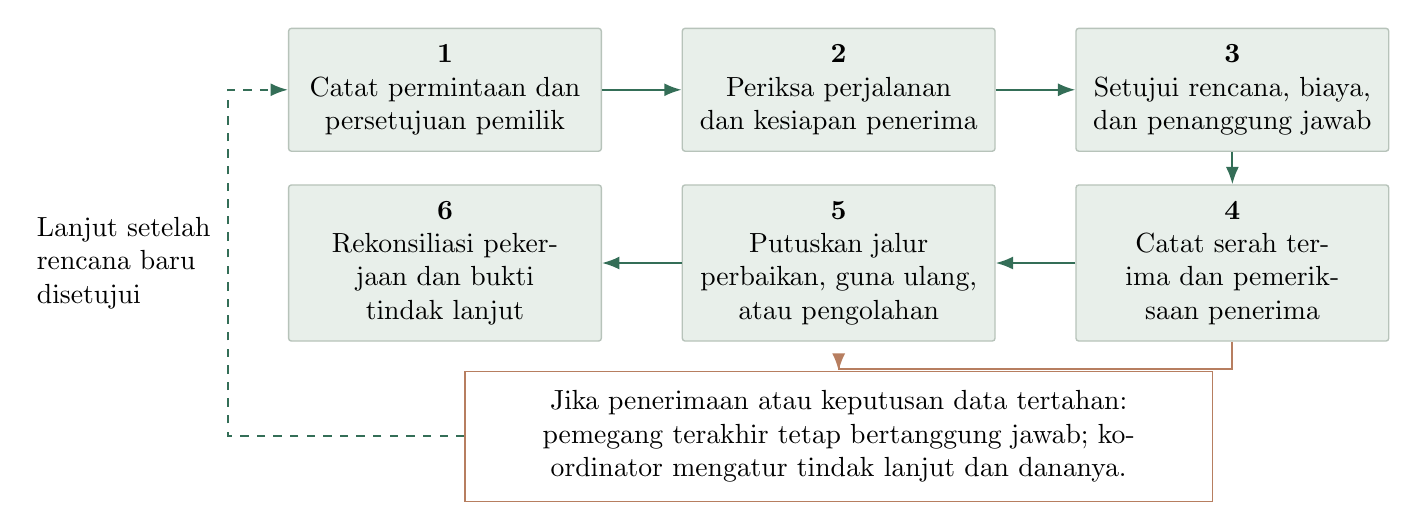
\begin{tikzpicture}[box/.style={draw=rule,line width=.5pt,fill=sage,rounded corners=1pt,text width=3.55cm,minimum height=1.1cm,align=center,inner sep=6pt},edge/.style={-{Latex[length=2.2mm]},draw=forest,line width=.7pt}]
\node[box] (s0) at (0,0) {\textbf{1}\par Catat permintaan dan persetujuan pemilik};
\node[box] (s1) at (5,0) {\textbf{2}\par Periksa perjalanan dan kesiapan penerima};
\node[box] (s2) at (10,0) {\textbf{3}\par Setujui rencana, biaya, dan penanggung jawab};
\node[box] (s3) at (10,-2.2) {\textbf{4}\par Catat serah terima dan pemeriksaan penerima};
\node[box] (s4) at (5,-2.2) {\textbf{5}\par Putuskan jalur perbaikan, guna ulang, atau pengolahan};
\node[box] (s5) at (0,-2.2) {\textbf{6}\par Rekonsiliasi pekerjaan dan bukti tindak lanjut};
\draw[edge] (s0) -- (s1);
\draw[edge] (s1) -- (s2);
\draw[edge] (s2) -- (s3);
\draw[edge] (s3) -- (s4);
\draw[edge] (s4) -- (s5);
\node[draw=clay,fill=white,text width=9cm,align=center,inner sep=7pt] (held) at (5,-4.4) {Jika penerimaan atau keputusan data tertahan: pemegang terakhir tetap bertanggung jawab; koordinator mengatur tindak lanjut dan dananya.};
\draw[edge,draw=clay] (s3.south) -- ++(0,-.35) -| (held.north);
\draw[edge,dashed] (held.west) -- ++(-3,0) |- node[pos=.25,left,text width=2.3cm,align=left] {Lanjut setelah rencana baru disetujui} (s0.west);
\end{tikzpicture}
}

\end{document}
